% Research Background Chapter
\subsection{Background and Motivation}

Radar technology has long been associated with vehicles, military radar, weather forecasting, and simple target tracking. However, this technology has not been as widely researched in the field of robotics as sensors with shorter wavelengths, such as cameras or LiDAR operating in the optical range.

In recent years, new models of ‘4D imaging’ radars have appeared on the market, primarily intended for autonomous vehicles. Sensors such as the Arbe LRR610 chipset, radar components, see Figure \ref{fig:Arbe-4D-radar}, for example, have 48 transmitting and 48 receiving antennas (2304 virtual channels) and provide an angular resolution of less than 1\degree at a range of 350 m. This enables the detection of pedestrians and objects at distances that are unattainable with cameras and LiDAR modules, which also fail to perform well in adverse operating conditions\citep{arbe_radar_processor, idtechex_automotive_radar}.

\begin{figure}[H]
    \centering
    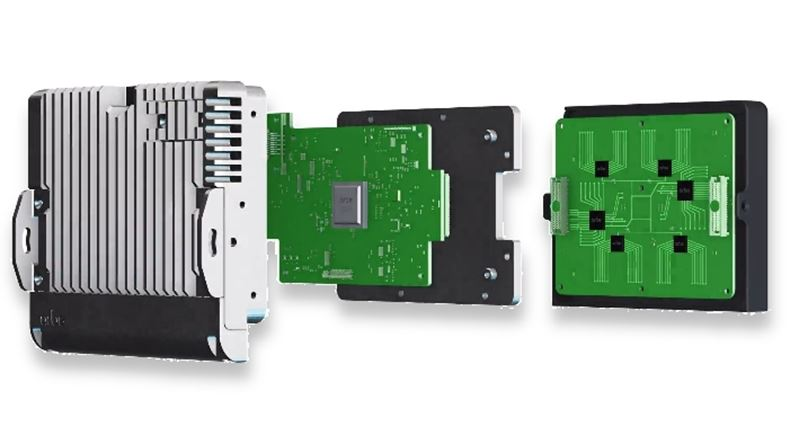
\includegraphics[width=0.75\linewidth]{Src/images/Arbe 4D radar.jpg}
    \caption{Arbe 4D radar}
    \label{fig:Arbe-4D-radar}
\end{figure}

It is great when such models become available on the market, but such high performance and high detection resolution come at the price of complexity and, accordingly, the cost of all the equipment: for example, a single radar with a 48 × 48 MIMO array can currently cost more than the entire platform of a small robot, including motors, control boards, and much more, so it is rarely used for mobile robots \citep{arbe_radar_processor}.

\noindent
At the same time, the radar development industry is moving towards compact ‘radar-on-a-chip’ solutions that integrate everything from VCOs to ADCs and processor cores. These sensors use only 1–2 transmitting and 3–4 receiving antennas. Examples include the TI AWR2243 (see Fig. \ref{fig:AWR2243} (3 TX / 4 RX, 76–81 GHz) and Infineon BGT60TR13C (1 TX / 3 RX, 60 GHz). According to the manufacturers, the price of these chips when ordering more than 1,000 pieces is approximately equal to the price of a loaf of bread, which makes them affordable not only as IoT devices, but also for robots \citep{ti_awr2243_datasheet} \citep{ti_mmwave_overview} \citep{infineon_bgt60tr13c}.


\begin{figure}
    \centering
    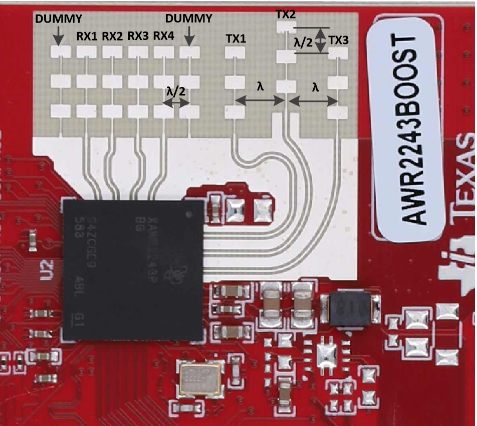
\includegraphics[width=0.3\linewidth]{Src/images/AWR2243.png}
    \caption{AWR2243 PCB board}
    \label{fig:AWR2243}
\end{figure}


Radars with limited functionality are found in various objects, from table lamps to smart speakers. For example, the FP2 home presence sensor \cite{Aqara_Presence_Sensor_FP2} demonstrates the ability to detect multiple people and their movements, offering an unobtrusive alternative to traditional surveillance methods.
In another area, mobile robotics is experiencing rapid growth, and its applications are expanding from industry to everyday life. Active work is underway to develop autonomous mobile robots for tasks in factories, disaster relief, support for the military-industrial complex, and space exploration.
Mobile robots are moving from closed test sites to real warehouses, factories, and city streets. There, they encounter a dynamic environment in which the trajectories of people, trucks, bicycles, scooters, and other robots are constantly changing. Any error in perception leads not to a ‘loss of position on the map,’ but to a real risk of injury.

\begin{table}[h]
    \centering
    \caption{Threat Categories and Potential Consequences}
    \label{tab:threats_consequences}
    \begin{tabular}{|>{\raggedright\arraybackslash}m{2.5cm}|>{\raggedright\arraybackslash}m{6cm}|>{\raggedright\arraybackslash}m{6.5cm}|}
        \hline
        \textbf{Category} & \textbf{Examples of Threats} & \textbf{Potential Consequences} \\ \hline
        \textbf{People} & Pedestrian, forklift operator, cyclist & Injuries, fatalities, reputational losses \\ \hline
        \textbf{Transport} & Car, forklift truck, AMR cart & Equipment damage, production line downtime \\ \hline
        \textbf{Animals} & Robot dogs, service animals, wild animals & Unpredictable trajectory, social resonance \\ \hline
        \textbf{Other Robots} & Cooperative or foreign platforms & Resonance impacts, "robots block the way" \\ \hline
        \textbf{Falling Cargo} & Pallets, boxes, construction elements & Route obstruction, shelf collapse \\ \hline
    \end{tabular}
\end{table}
When considering general statistics:
\paragraph{USA data:}
\begin{itemize}
     \item Analysis of \textbf{37 OSHA investigations} shows that since 2011, there have been at least \textbf{20 fatalities} in the United States involving workers being struck or trapped by a robotic manipulator or mobile platform \citep{osha_robot_accidents};
    \item With regard to warehouse AMRs (Autonomous Mobile Robots), the study ‘Robot-related injuries’ recorded \textbf{27 injuries} over a three-year period resulting from attacks by mobile robots \citep{SANDERS2024104324};
\end{itemize}

\paragraph{Data for Europe:} Information on injuries and incidents involving mobile robots in warehouses, factories, and city streets is less centralised than in the United States, where\textbf{ despite this, OSHA publishes} detailed reports in Europe. Using available sources and taking into account the request for similar data.
\begin{itemize}
\item The European Agency for Safety and Health at Work has estimated\textbf{20-25 serious incidents} involving robots each year in the \textbf{EU}, of which \textbf{approximately 30\% are related to mobile platforms}. Fatalities are quite rare (<1\%), but collisions and injuries from entrapment predominate. \citep{oshaeu_robotics2023}.
The European Foundation for the Improvement of Living and Working Conditions documented 15 cases of injuries involving robots in warehouses and factories in the EU between 2018 and 2022. Most cases were related to poor synchronisation between humans and robots, with Germany (one of the leaders in the use of robots in manufacturing) accounting for up to 40\% of incidents, often involving AGVs (Automated Guided Vehicles)
.
radio1943detection\end{itemize}

\noindent

\noindent
This brings us back to the original problem: the navigation module must sequentially identify and classify moving objects (see Table \ref{tab:threats_consequences}), while the planner must predict their future location; failure to do so increases the likelihood of accidents and associated legal costs.

When planning a route, the speed and direction of each object must be taken into account, and often a static ‘cloud of points’ is not sufficient \citep{s24113573}.


\begin{figure}[H]
    \centering
    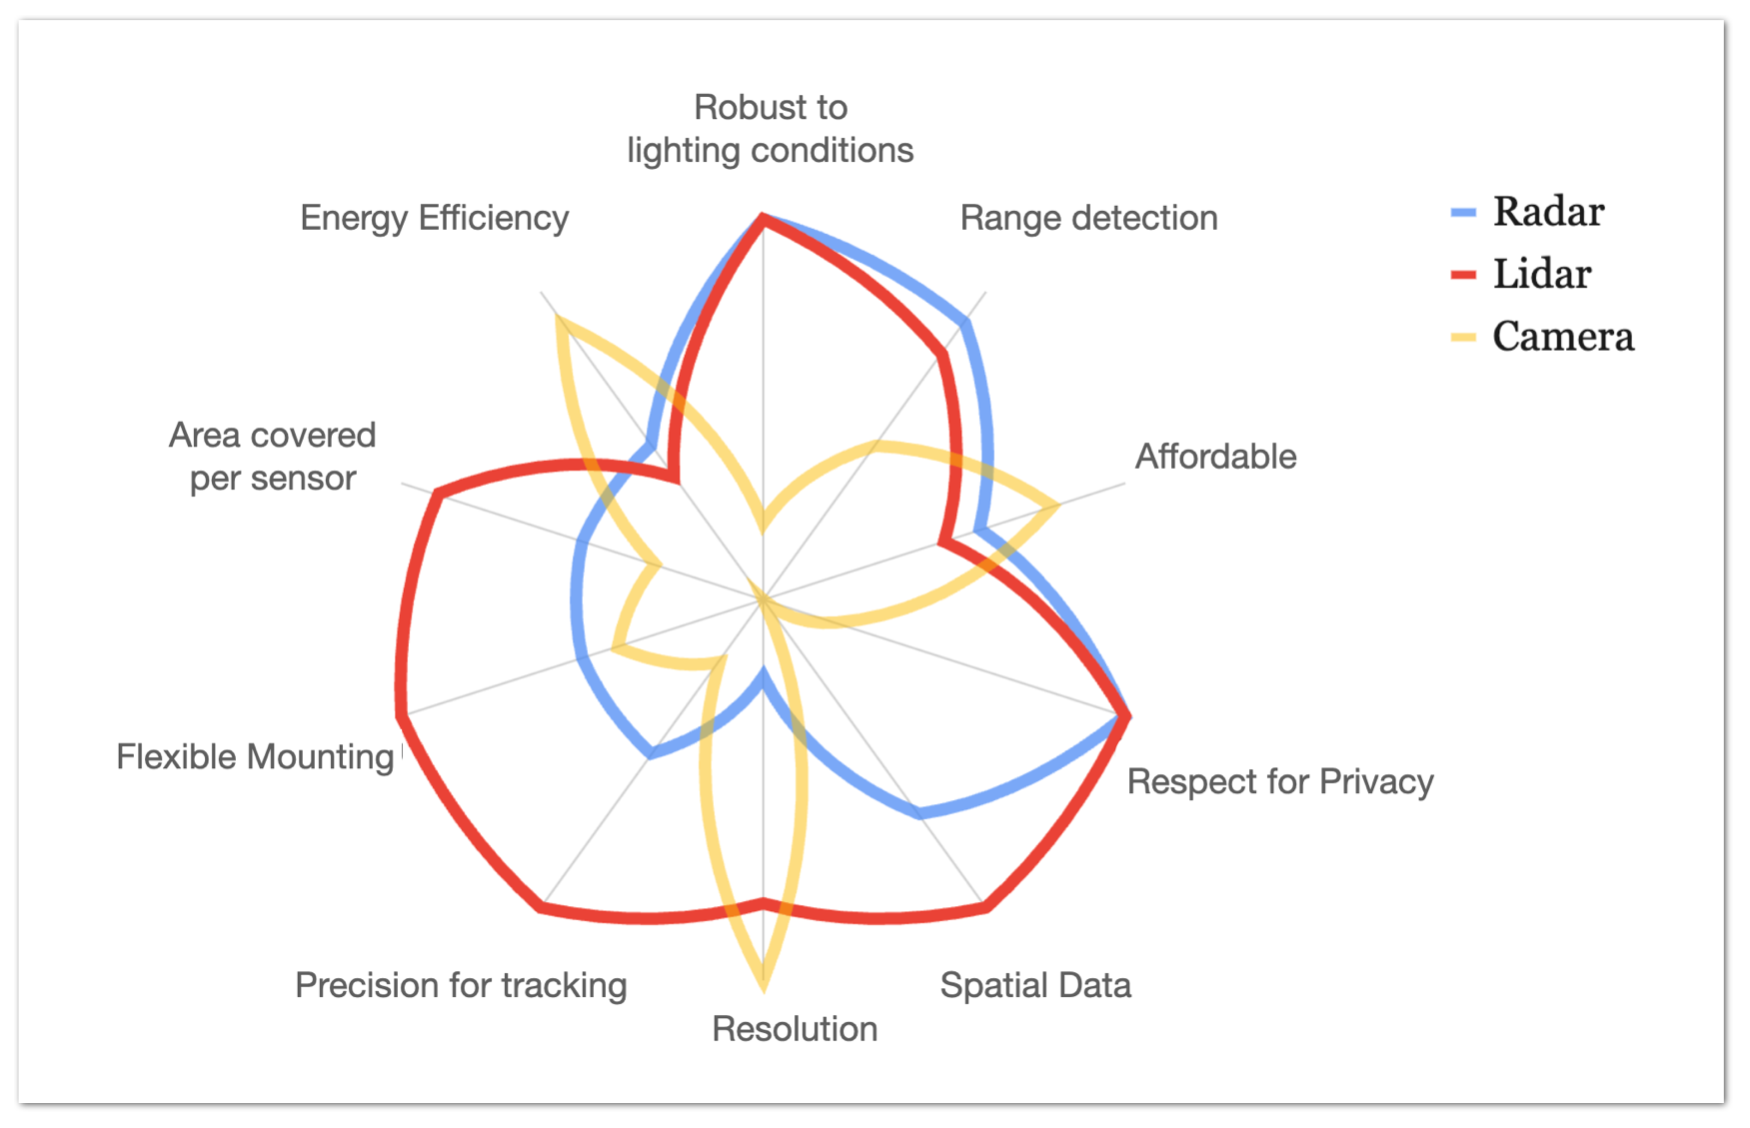
\includegraphics[width=0.6\linewidth]{Src//images/Sensors-comparison.png}
    \caption{Comparison of different sensor types}
    \label{fig:sensor_comp}
\end{figure}

In a world where radar is becoming the sensor technology of choice for information systems, it offers a number of advantages that are ideal for managing complex dynamic environments. Unlike cameras, which struggle in poor lighting or are hampered by factors such as dust, fog, rain or snow, millimetre-wave radar provides stable, high-resolution sensing regardless of weather or environmental conditions; see Fig. \ref{fig:sensor_comp}. In addition, their ability to penetrate objects and detect through certain materials, such as plastic or plasterboard, provides a significant advantage in challenging conditions. This ability allows data sensors of these types to recognise their environment with greater accuracy and foresight to detect objects.



\begin{figure}[H]
    \centering
    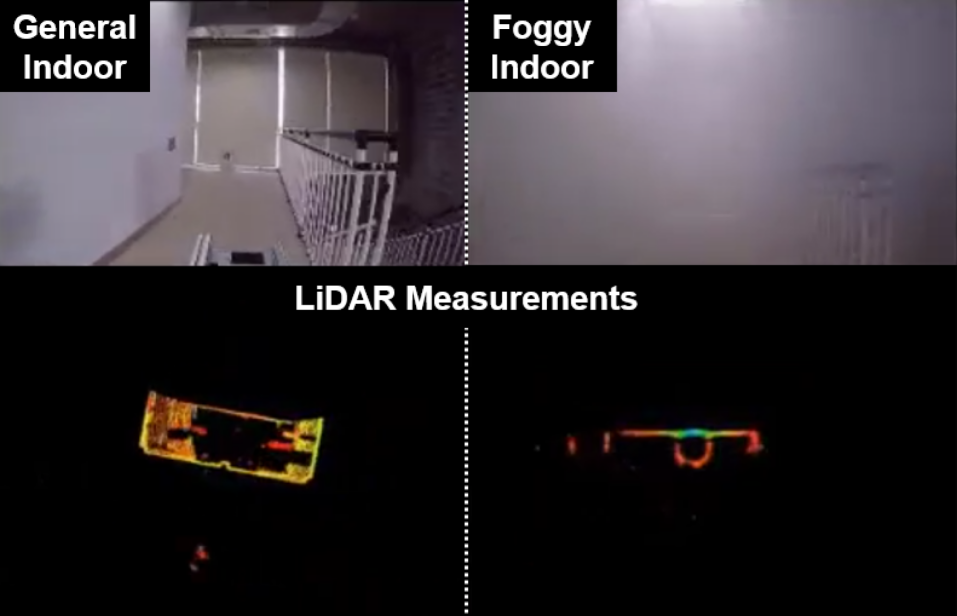
\includegraphics[width=0.75\linewidth]{Src/images/x1.png} 
    \caption{Lidar measurements in a foggy indoor environment \citep{harlow2021mmwave}}
    \label{fig:lidarfogy}
\end{figure}


Navigation situations and cases that seriously affect the operation of cameras \citep{starr2013navigation} and lidars \citep{Skolnik2001}, as shown in Figure \ref{fig:lidarfogy}, but do not significantly affect the operation of radars. Theoretically, radars can even pass through not only various materials, but also small solid particles, due to the use of longer waves.
Radar systems transmit and receive specially formed electromagnetic pulses to determine the distance and direction of objects, offering advanced sensor probing capabilities. Thus, radar as a sensor for information systems makes it a valuable option for integration into existing systems or as a standalone sensor, enabling both metric and semantic tasks to be performed.






% % Настоящий раздел излагает ключевые теоретические основы, лежащие в центре применения миллиметрового FMCW‐радара для планирования движения мобильного робота в динамичной среде. Материал охватывает (i) принципы радиолокации в диапазоне 60–64 ГГц, (ii) методы вероятностного представления среды и отслеживания препятствий, а также (iii) алгоритмические подходы к локальному планированию траектории, учитывающие высокоскоростную динамику целей.

% 

% Consequently, the development of mobile robots is not only commercially viable and scientifically valuable but also represents a crucial strategic initiative for nations and society as a whole. The history of their evolution, marked by increasing speeds and diverse applications, reflects the broader achievements in robotics \citep{turn0search0}. This progress, particularly the increasing speed of mobile robots, inevitably leads to greater demands on their internal systems, including actuators, sensor accuracy, and control algorithms.

% Traditionally, robotic systems have relied heavily on light-based sensors such as cameras and LiDARs to build a representation of their environment. However, these sensors face functional limitations, especially in challenging conditions like poor illumination or when dealing with structurally degraded scenes. Despite ongoing developments in areas like photometric calibration \citep{PointLightYang} and camera distortion calibration \citep{Jin2019}, these sensors are not universally effective.


% % \scriptsize
% % \begin{longtable}{|l|l|c|c|c|c|c|c|c|c|}
% % \caption{Capabilities and basic sensor information}
% % \\
% % \hline
% % \textbf{Sensor} & \textbf{Data Type} & \textbf{Range} & \textbf{Density} & \textbf{Res.} & \textbf{Rng} & \textbf{Ang} & \textbf{Vel} & \textbf{Dark} & \textbf{VDE} \\
% % \hline
% % Cameras & 2D Images & Medium & Dense & High & Yes* & Yes* & No & Limited & Limited \\
% % Depth Sensors & Depth Maps & Short & Dense & High & Yes & Yes & No & Full & Occluded \\
% % Lidar & 3D Point Clouds & Long & Sparse & High & Yes & Yes & No & Full & Occluded \\
% % 2D Scanning Radar & Polar Range Map & Long & Dense & High & Yes & Yes & No & Full & Full \\
% % 3D SoC Radar & Spectral Heatmap & Long & Dense & Medium & Yes & Yes & Yes & Full & Full \\
% % 3D SoC Radar & 3D Point Clouds & Long & Very Sparse & Low & Yes & Yes & Yes & Full & Full \\
% % \hline
% % \end{longtable}
% % \normalsize

% In this context, millimeter-wave (mmWave) radar is emerging as a transformative sensing technology for mobile robots. It offers a unique set of advantages particularly well-suited to the complexities of dynamic environments. Unlike cameras that struggle in low light or are hindered by obscurants like dust, fog, or rain, mmWave radar provides reliable, high-resolution sensing across a wide range of weather and environmental conditions (Source 2.2, 2.4, 2.5). Furthermore, its ability to penetrate and detect objects through certain obstacles, such as plastic or drywall, gives it a significant advantage in cluttered and complex spaces (Source 2.1, 2.2). This allows mobile robots to perceive their surroundings with enhanced accuracy and foresight.

% Navigating and planning motion in dynamic settings presents a formidable challenge for autonomous systems (Source 3.2, 3.5). Unexpected obstacles, the movement of people, and the presence of other robots necessitate constant re-evaluation of paths and instantaneous decision-making (Source 3.1, 3.3). Traditional sensors, with their inherent limitations, may not provide sufficiently rich or timely data to cope with these complexities, potentially leading to hesitant or unsafe robot behavior (Source 3.4).




\subsection{Problem Statement}

There are several reasons why millimeter wave radars are not commonly utilized in robotics. Similar to other sensors, radar presents many issues that must be addressed when developing new solutions. Notably, radar possesses unique noise characteristics such as false reflections that occur outside the sensor's range, more complex speckle noise, and multipath reflections, which result in multiple reflections from a single object.

However, the vast majority of projects use these radars in a ‘lidar-like’ manner: reflections are turned into sparse point clouds and then apply SLAM, mapping and deep learning algorithms originally developed for lidar density and isotropy \citep{10919654}. 

This straightforward adaptation raises several fundamental problems. First, radar clouds are two orders of magnitude rarer than lidar clouds and distorted by multipath ‘ghosts’, forcing the introduction of a heavy cascade of detections, clustering and tracking before the data are suitable for geometric problems at all \citep{Wu2025DiffusionBasedMP}.
Second, the unique attributes of radar, instantaneous Doppler velocity, phase, SNR, are discarded in such pipelines, although they can improve the prediction of obstacle dynamics. Attempts to 'complete' lidar-oriented networks through post-super-resolutions\citep{10161429}

\noindent
Despite this, radars have the following features:
\begin{itemize}
    \item Operates in poor visibility conditions (dust, smoke, fog, darkness);
    \item Provides distance measurements;
    \item Enables velocity estimation of objects using the Doppler effect;
    \item Offers a wide field of view due to broad antenna beamwidth;
    \item Insensitive to ambient lighting and surface color;
    \item Supports multi-channel reception (multiple Rx antennas), allowing angular estimation and 2D/3D scene reconstruction.
\end{itemize}

This raises a key research question: \emph{Is it possible to sacrifice some angular resolution in order to use inexpensive radars on robots where weight and cost are critical?}



    
\subsection{Research Aim and Objectives}

\paragraph{Aim of this work} To investigate the feasibility of using an mmWave radar as a sensor for the information system of a mobile robot in a dynamic environment.

\paragraph{Research Objectives} An information system to detect and predict the motion of the object, allowing the robot to plan its trajectory.

\paragraph{Research Subject}
Integration of FMCW mmWave radar for path adjustment of mobile robots in dynamic indoor environments.



%%%%%%%%%%%%%%%%%%%%%%%%%%%%%%%%%%%%%%%%%%%%%%%%%%%%%%%%%%%%%%%%%%%%%%%%%%%%%%%%%%%%%%
\subsection{Research Questions and Hypotheses}

\\
\paragraph{Research Questions:}

\begin{enumerate}
    \item Is it possible to adapt the trajectory of a mobile robot based on data from a compact mmWave radar upon detecting moving objects in indoor environments?
    \item Are compact mmWave radars (24–60 GHz) in detecting and identifying biological objects, such as humans, under typical indoor conditions?
    \item Does the presence of low-reflectivity objects (textile or soft furniture) affect the robot's ability to detect them and adjust its trajectory accordingly?
\end{enumerate}

\paragraph{Hypotheses:}

\begin{enumerate}
    \item A single mmWave radar transmission-reception cycle is sufficient to detect an object and estimate its velocity for motion planning.
    \item  Despite limited angular resolution, variations in signal amplitude and Doppler spread allow classification of motion state (static vs. moving) of nearby obstacles.
\end{enumerate}




%%%%%%%%%%%%%%%%%%%%%%%%%%%%%%%%%%%%%%%%%%%%%%%%%%%%%%%%%%%%%%%%%%%%%%%%%%%%%%%%%%%%%%
\paragraph{Tasks}
To achieve the research goals and support the proposed hypotheses, the following key tasks have been identified. These tasks have been carefully organized in a logical sequence to ensure a smooth transition from theoretical analysis to practical application and evaluation:

\begin{enumerate}
  \item Analyse the relevance of mmWave radar for mobile-robot motion planning 
  \item Select suitable mmWave-radar hardware and key performance parameters
  \item Develop radar signal-processing algorithms
  \item Investigate detection of moving and stationary objects with the radar
  \item Test the motion-planning algorithms in a dynamic environment
   \item Design integration of the chosen radar into the robot platform

  \item Analysis of research results
\end{enumerate}


%%%%%%%%%%%%%%%%%%%%%%%%%%%%%%%%%%%%%%%%%%%%%%%%%%%%%%%%%%%%%%%%%%%%%%%%%%%%%%%%%%%%%%
\textbf{Scope and Delimitations} 
\noindent
This reserch primarily investigates the potential and practical application of FMCW mmWave radar \textbf{(operating in the 60-64 GHz band)} for mobile robot in dynamic environments. Particular attention is given to how these features affect detection in robotic systems.

The study includes the selection and integration of radar hardware, design of signal processing pipelines, and include of tracking methods to radar data. These elements are tested in the context of local navigation through moving and stationary obstacles.

\medskip
Research is limited to short-range detection up to \textbf{10 meters} or shorter in structured and semi-structured indoor environments. The experimental setup is based on a differential drive robot equipped with a single forward-facing radar unit.

\noindent
The delimitations of this study are as follows:

\begin{itemize}
  \item The primary focus is on exploring the capabilities and limitations of \textbf{mmWave radar sensing}, rather than system-level integration with global SLAM or decision-making modules.

  \item The system utilizes only \textbf{radar} and \textbf{inertial/odometric} data, deliberately excluding other common sensors such as \textbf{LiDAR}, \textbf{vision}, or \textbf{ultrasound}.

  \item Navigation is constrained to ground-level interaction; the detection of elevated, suspended, or multilevel obstacles is outside the scope.

  \item Robot motion is limited to moderate speeds (\textbf{1--2 m/s}) and assumes interaction with \textbf{non-aggressive dynamic objects}, such as humans or other robots in shared indoor spaces.

  \item Broader system-level concerns such as multi-agent coordination, semantic understanding, or complex decision-making frameworks are not addressed in this work.
\end{itemize}


\subsection{Research Design/Approach}
The main objective of this study is to evaluate the applicability of low-cost millimeter-wave radars for motion planning of a mobile robot in a dynamic indoor environment.

\begin{itemize}
\item \textbf{Stages.} (1) Experimental testing in real conditions;(2) Evaluation of the radar's penetration capability and visibility of various objects in the environment; (3) Design and implementation of object detection or classification algorithms; (4) Development of radar integration with the robot and data interface; 

\item \textbf{Research methodology:}
\begin{itemize}
\item \textbf{Comparative analysis of technical parameters.}
Compare the key characteristics (range resolution, angular accuracy, update rate, power consumption) of various radar modules relevant to the mobile robot platform.
\item \textbf{Analytical calculation method.}
Based on radar equations and kinematic constraints of the robot, derive theoretical limits for the detection range and speed determination of objects. These calculations serve as a guideline for selecting parameters (chirp angle, pulse repetition interval PRI), as well as for data processing and presentation.

\item \textbf{Experimental method.}
Controlled tests were conducted in a room where the robot followed a predetermined path, encountering static and dynamic obstacles during its movement. Radar data was recorded and then processed to calculate detection performance.
\end{itemize}
\end{itemize}




%%%%%%%%%%%%%%%%%%%%%%%%%%%%%%%%%%%%%%%%%%%%%%%%%%%%%%%%%%%%%%%%%%%%%%%%%%%%%%%%%%%%%%


